\documentclass[tikz]{standalone}


\usetikzlibrary{shapes, shapes.geometric, shapes.misc, shapes.arrows}
%\usetikzlibrary{3d, perspective}
\usetikzlibrary{arrows, arrows.meta}
\usetikzlibrary{angles, math, calc, matrix}
\usetikzlibrary{positioning}
%\usetikzlibrary{fadings, shadows, shadings}
\usetikzlibrary{decorations.pathreplacing, decorations.markings, decorations.text, calligraphy}
%\usetikzlibrary{circuits.ee.IEC}

\begin{document}

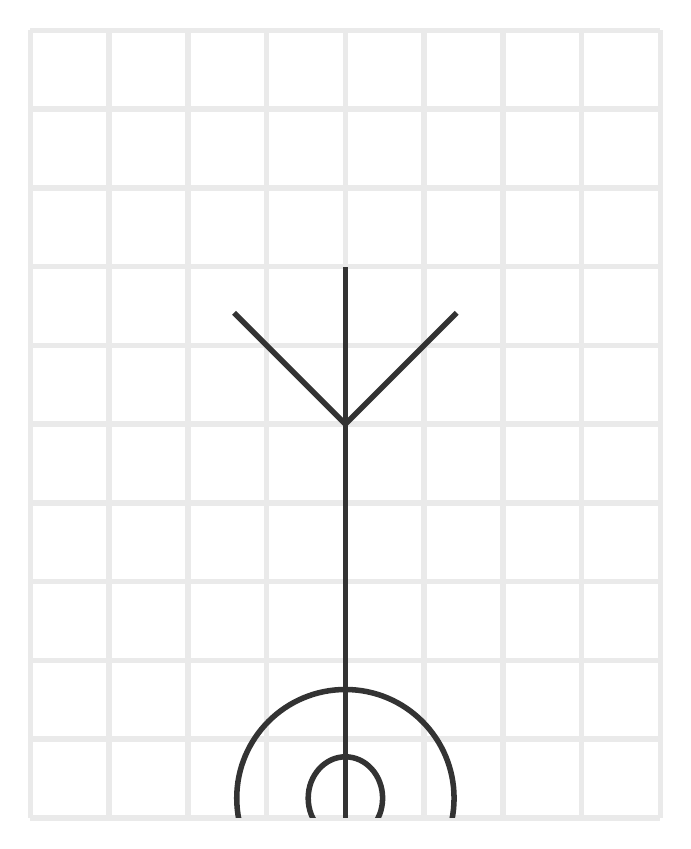
\begin{tikzpicture}[black!80, line width = 2pt]

    \def\Ybound{10}
    \def\Xbound{4}

    \draw[opacity = 0.1] (-\Xbound,-0) grid (\Xbound,\Ybound);
    \clip (-\Xbound,-0) rectangle (\Xbound,\Ybound);

    \def\nuclea{0.35}
    \def\radius{2.3}

    \coordinate (O) at (0,0.25);
    


    \begin{scope}[scale = 0.60, transform shape]
        \draw (O) circle (\radius);
        \draw[rounded corners, rotate = 90]  
                (O) ellipse [x radius= 2.5*\nuclea , y radius= 2.25*\nuclea ];
    \end{scope}
    
    \draw (0,0) -- (0,7);
    \draw foreach \SIGN in {-, +} {(0,5) -- ([turn]\SIGN 45:2)};

\end{tikzpicture}

\end{document}